\section{Evaluation}\label{sec:evaluation}

We now evaluate the tightness, time complexity and output size of routing function, pipeline characterization, and the main factors of realization numerically. All experiments are conducted on a 1.6 GHz Intel Core i5 with 4 GB RAM.

%We now evaluate the characterization of a routing function and a pipeline from the tightness, computation complexity, and output size.  and running OS X system.

\subsection{Routing Function Characterization Tightness}
\label{sec:eval1}

We demonstrate the tightness of characterization of a routing function by comparing the $ec(M)$, the number of equivalent classes for a set of matches $M$, from two mappings (\ie, $\tau$ and $\tau_G$) for several routing functions. The computation of $ec(M)$ for the mapping $\tau$ is based on the definition of f-equivalence which will get the exact value of the number of equivalent classes for a set of matches $M$ for a particular routing function. The routing functions we use are shown as follows :

{\small
\begin{verbatim}
//  Routing function: simpleRoute
L0: def simpleRoute(Addr srcIP, Addr dstIP):
L1:   srcSw = hostTbl[srcIP]
L2:   dstSw = hostTbl[dstIP]
L3:   route = routeTbl[srcSw, dstSw]
L4:   return route
\end{verbatim}
}

Our first function, \texttt{simpleRoute} maps a packet's \texttt{srcIP} and \texttt{dstIP} to their host packet switches \texttt{dstSw} and \texttt{srcSw} based on a key-value table \texttt{hostTbl}. After that, \texttt{simpleRoute} gets the route from another table, \texttt{routeTbl}, where the key is two internal variables, \texttt{srcSw} and \texttt{dstSw}.

%Function 1 (\texttt{simpleRoute}) reads two inputs and maps them to internal variables respectively based on a table, \texttt{hostTbl}. After that, \texttt{simpleRoute} gets the route from another table, \texttt{routeTbl}, where the key is two internal variables.

{\small
\begin{verbatim}
//  Routing Function: condRoute
L0: condRoute(srcIP, dstIP):
L1:   srcSw = hostTbl[srcIP]
L2:   dstSw = hostTbl[dstIP]
L3:   routeCond = condTbl[srcIP, dstIP]
L4:   route = routeTbl[srcSw, dstSw, routeCond]
L5:   return route
\end{verbatim}
}

Our second function \texttt{condRoute} extends \texttt{simpleRoute} by introducing a route condition variable (\ie, \texttt{routeCond}) which is computed by a condition table, \texttt{condTbl}. After that, \texttt{condRoute} computes the route from three internal variables, 
\texttt{srcSw}, \texttt{dstSw}, and \texttt{routeCond}.

%Function 2 (\texttt{f2}) is similar to \texttt{simpleRoute} except that there is a third table, \texttt{condTbl}, which returns an internal variable, \texttt{cond}, used as a part of the key of \texttt{routeTbl}.

{\small
\begin{verbatim}
//  Routing Function: secureRoute
L0: secureRoute(Addr srcIP, Addr dstIP):
L1:   if (isFiltered(srcIP)):
L2:     return Drop()
L3:   else:
L4:     route = fwdTbl[dstIP]
L5:     return route
\end{verbatim}
}

Our third function \texttt{secureRoute} drops all traffic from \texttt{srcIP}s on a filter list (\ie, \texttt{isFiltered}) and forwards remaining traffic based on the table \texttt{fwdTbl} by only matching \texttt{dstIP}.

As our final function, we consider the example function \texttt{onPkt} as shown in Sec.~\ref{sec:model-and-main-results}
%\begin{verbatim}
%\\  Routing function: onPkt
%    Map hostTbl[key: dstIP, value: switch]
%    Map condTbl[key: (dstIP, port), value: cond]
%    Map routeTbl[key: (switch, cond), value: outPort]
%L0: onPkt(Type ethType, Addr srcIP, Port srcPort, \
%          Addr dstIP, Port dstPort):
%L1: if (ethType != IPv4):
%L2:   return Drop()
%L3: if (verify(srcPort, srcIP)):
%L4:   dstCond = condTbl[dstIP, dstPort]
%L5:   dstSw = hostTbl[dstIP]
%L6:   return Forward(port = routeTbl[dstCond, dstSw])
%L7: return Drop()
%\end{verbatim}

\para{Results:} We present our results in Table~\ref{table:table1}. Specifically, in Table~\ref{table:table1}, column 2 defines the domain of \texttt{srcIP}, \texttt{dstIP}, columns 3-6 give the output ranges $O(tbls)$ of each table, and columns 7-10 give the values of selected fields in each function's $\tau(f)$ and $\tau_G(f)$. 

%We present our results in Table~\ref{table:table1}. Specifically, in Table~\ref{table:table1}, column 2 defines the domain of \texttt{srcIP}, \texttt{dstIP}, columns 3-6 give the output ranges $O(tbls)$ of each table, and columns 7-10 give the values of selected fields in each function's $\tau(f)$ and $\tau_G(f)$. 

Note that the notation $b1(\texttt{scR})$ represents the branch 1 in \texttt{scR}, \ie, L1$\to$L2, while $b2(\texttt{scR})$ represents the branch 2 in \texttt{f3}, \ie, L1$\to$L3$\to$L4$\to$L5. We record N/A when a value is not applicable to a given function, and null for values of $\tau(f)$ where computation failed to halt. And we only evaluate the equivalent class value in the output vector of characterization of a function.

%Given the characterization results for the four functions, \texttt{simpleRoute}, \texttt{f2}, \texttt{f3}, and \texttt{onPkt}. The second column, $bits(input)$, defines the number of bits of both inputs, \ie, \texttt{srcIP}, \texttt{dstIP}; We use $\#O(t)$ to represent the number of possible output value for the table $t$; We only evaluate the equivalent class value in the output vector of characterization of a function for a particular input; The notation $b1(\texttt{f3})$ represents the branch 1 in \texttt{f3}, \ie, L1$\to$L2, while $b2(\texttt{f3})$ represents the branch 2 in \texttt{f3}, \ie, L1$\to$L3$\to$L4$\to$L5.

In our evaluation of \texttt{smplR} and \texttt{condR}, the results of $\tau$ and $\tau_G$ are almost identical in every case barring an extreme one where $O(\texttt{condTbl})$ = 1. Notably, our values of $\tau(f)$ and $\tau_G(f)$ are not influenced by the range of \texttt{routeTbl} (\ie, $O(\texttt{routeTbl})$), which can be observed from the first three rows in the table. This implies there is no pattern between the allocation of routes to (\texttt{srcIP}, \texttt{dstIP}) pairs $\tau(f)$ can exploit to reduce its number of equivalence classes. Considering $s_1$ and $s_2$ as two values of \texttt{srcIP}, if \texttt{hostTbl}($s_1$) is not equal to \texttt{hostTbl}($s_2$), then the chance of $s_1 \sim_f s_2$ is very small.

%From the evaluation of simpleRoute and f2, we can see the result of $\tau$ and $\tau_G$ are almost the same except an extreme case where $\#O(\texttt{condTbl})$ = 1. Also, the results are not influenced by $\#O(\texttt{routeTbl})$, which can be observed from the first three rows in the table. This is because, considering $s_1$ and $s_2$ as two values of $srcIP$, if \texttt{hostTbl}($s_1$) is not equal to \texttt{hostTbl}($s_2$), then the chance of $s_1 \sim_f s_2$ is very small.

Further notice that our functions with control statements: \texttt{secureRoute} and \texttt{onPkt} have a large gap between $\tau$ and $\tau_G$, suggesting $\tau_G$'s bound is loose on heavily branching programs. However, as rows b1(scR) and b2(scR) show, we can ameliorate this problem by calculating each route through a program characteristic function separately. For each branch, the result of $\tau$ and $\tau_G$ maintains the tightness, which is shown in the rows with $b1(\texttt{scR})$ and $b2(\texttt{scR})$ in Table~\ref{table:table1}. Also, we evaluate the example routing function \texttt{onPkt}, and the result is shown in the last row in the table. Need to mention that, both $\tau(f)$(\texttt{srcIP}) and $\tau(f)$(\texttt{dstIP}) are null means that the computation time is too long to compute the result.

%For the functions with control statements, such as f3, the results of $\tau$ and $\tau_G$ have a large gap. However, in this case, we can split the function into different branches. For each branch, the result of $\tau$ and $\tau_G$ maintains the tightness, which is shown in the rows with $b1(\texttt{f3})$ and $b2(\texttt{f3})$ in Table~\ref{table:table1}. Also, we evaluate the example routing function \texttt{onPkt}, and the result is shown in the last row in the table. Need to mention that, both $\tau$(f)(\texttt{srcIP}) and $\tau$(f)(\texttt{dstIP}) are null means that the computation time is too long to compute the result.

\begin{table*}[t]
\centering
\scalebox{0.6}{
\begin{tabular}{ | l | l | l | l | l | l | l | l | l | l | }
    \hline
    $f$ & $bits(IP)$ & $O(\texttt{hostTbl})$ & $O(\texttt{routeTbl})$ & $O(\texttt{condTbl})$ & $O(\texttt{fwdTbl})$ & $\tau$(f)(\texttt{srcIP}) & $\tau$(f)(\texttt{dstIP}) & $\tau_G$(f)(\texttt{srcIP}) & $\tau_G$(f)(\texttt{dstIP}) \\
    \hline   
    smplR & 10 & 100 & 2 & N/A & N/A  & 100 & 100 & 100 & 100 \\
    smplR & 10 & 100 & 30 & N/A & N/A & 100 & 100 & 100 & 100 \\
    smplR & 10 & 100 & 5000 & N/A & N/A & 100 & 100 & 100 & 100 \\
    smplR & 12 & 100 & 30 & N/A & N/A & 100 & 100 & 100 & 100 \\
    smplR & 10 & 200 & 30 & N/A & N/A & 200 & 200 & 200 & 200 \\
    condR & 10 & 100 & 30 & 50 & N/A & 1024 & 1024 & 1024 & 1024 \\
    condR & 10 & 100 & 30 & 5 & N/A & 1024 & 1024 & 1024 & 1024 \\
    condR & 10 & 100 & 30 & 1 & N/A & 100 & 100 & 1024 & 1024 \\
    scR & 10 & N/A & N/A & N/A & 100 & 2 & 100 & 2 & 1024 \\
    b1(scR) & 10 & N/A & N/A & N/A & N/A & 1 & N/A & 1 & N/A \\
    b2(scR) & 10 & N/A & N/A & N/A & 100 & 1 & 100 & 1 & 100 \\
    \texttt{onPkt} & 32 & 100 & 30 & 50 & N/A & null & null & $2^{32}$ & $2^{32}$ \\
    \hline
  \end{tabular}
  }
\vspace{1mm}
\caption{Characterization results of routing functions with different statistics.}
\label{table:table1}
\end{table*}


\subsection{Routing Function Characterization Time Complexity}
%We now compare the time required to compute $\tau$ and $\tau_G$ for given routing functions. We run our tests using \texttt{simpleRoute} where $O(\texttt{hostTbl})$ = 100 and $O(\texttt{routeTbl})$ = 30.

We now examine the computing complexity of characterization of a routing function by comparing the computation time of two mappings (\ie, $\tau$ and $\tau_G$) for the same function. As the same with the first evaluation, the computation of $\tau$ is based on the definition of f-equivalence. We run our tests using \texttt{simpleRoute} where the size of \texttt{hostTbl} = 100 with different size of domain of input (\ie, the bits of input) and different size of \texttt{routeTbl}.

\para{Results:} Fig.~\ref{fig:eval-ct} shows the scalability of $\tau_G$ as input size and \texttt{routeTbl} size grows. Specifically, Fig.~\ref{fig:eval-ct:a} gives the result with fixed \texttt{routeTbl} size which equals 100, and Fig.~\ref{fig:eval-ct:b} gives the result with fixed input size which equals 6. As shown in Fig.~\ref{fig:eval-ct:a}, as the bit length of \texttt{srcIP} and \texttt{dstIP} increases, $\tau_G$'s computation time remains constant while $\tau$'s computation time grows in exponential order. And as illustrated in Fig.~\ref{fig:eval-ct:b}, as \texttt{routeTbl} size grows, the $\tau_G$'s computation time still remains constant while $\tau$'s computation time grows in polynomial level. This is because the computation of $\tau_G$ only requires the cuts of DFG which can be done in a very fast way but the computation of $\tau$ requires the execution of function for every possible input.

%$the computation time of $\tau_G$ has no change compared with the computation time of $\tau$ which grows rapidly.

%it requires large computation time based on the definition of f-equivalence to compute $\tau$ when the number of bits is large, while the computation of $\tau_G$ can be scalable with the number of bits of inputs (\ie, srcIP, dstIP) growing.

%We have examined the computing complexity of characterization of a routing function by comparing the computation time of two mappings (\ie, $\tau$ and $\tau_G$) for the same function. As the same with the first evaluation, the computation of $\tau$ is based on the definition of f-equivalence. We use \texttt{Function 1} as a target function with fixed table entries where $O(\texttt{hostTbl})$ = 100 and $O(\texttt{routeTbl})$ = 30 to do the evaluation. We have examined the computing complexity of characterization of a routing function by comparing the computation time of two mappings (\ie, $\tau$ and $\tau_G$) for the same function. As the same with the first evaluation, the computation of $\tau$ is based on the definition of f-equivalence. We use \texttt{Function 1} as a target function with fixed table entries where $O(\texttt{hostTbl})$ = 100 and $O(\texttt{routeTbl})$ = 30 to do the evaluation.

%\begin{figure}[tbh]
%    \centering
%    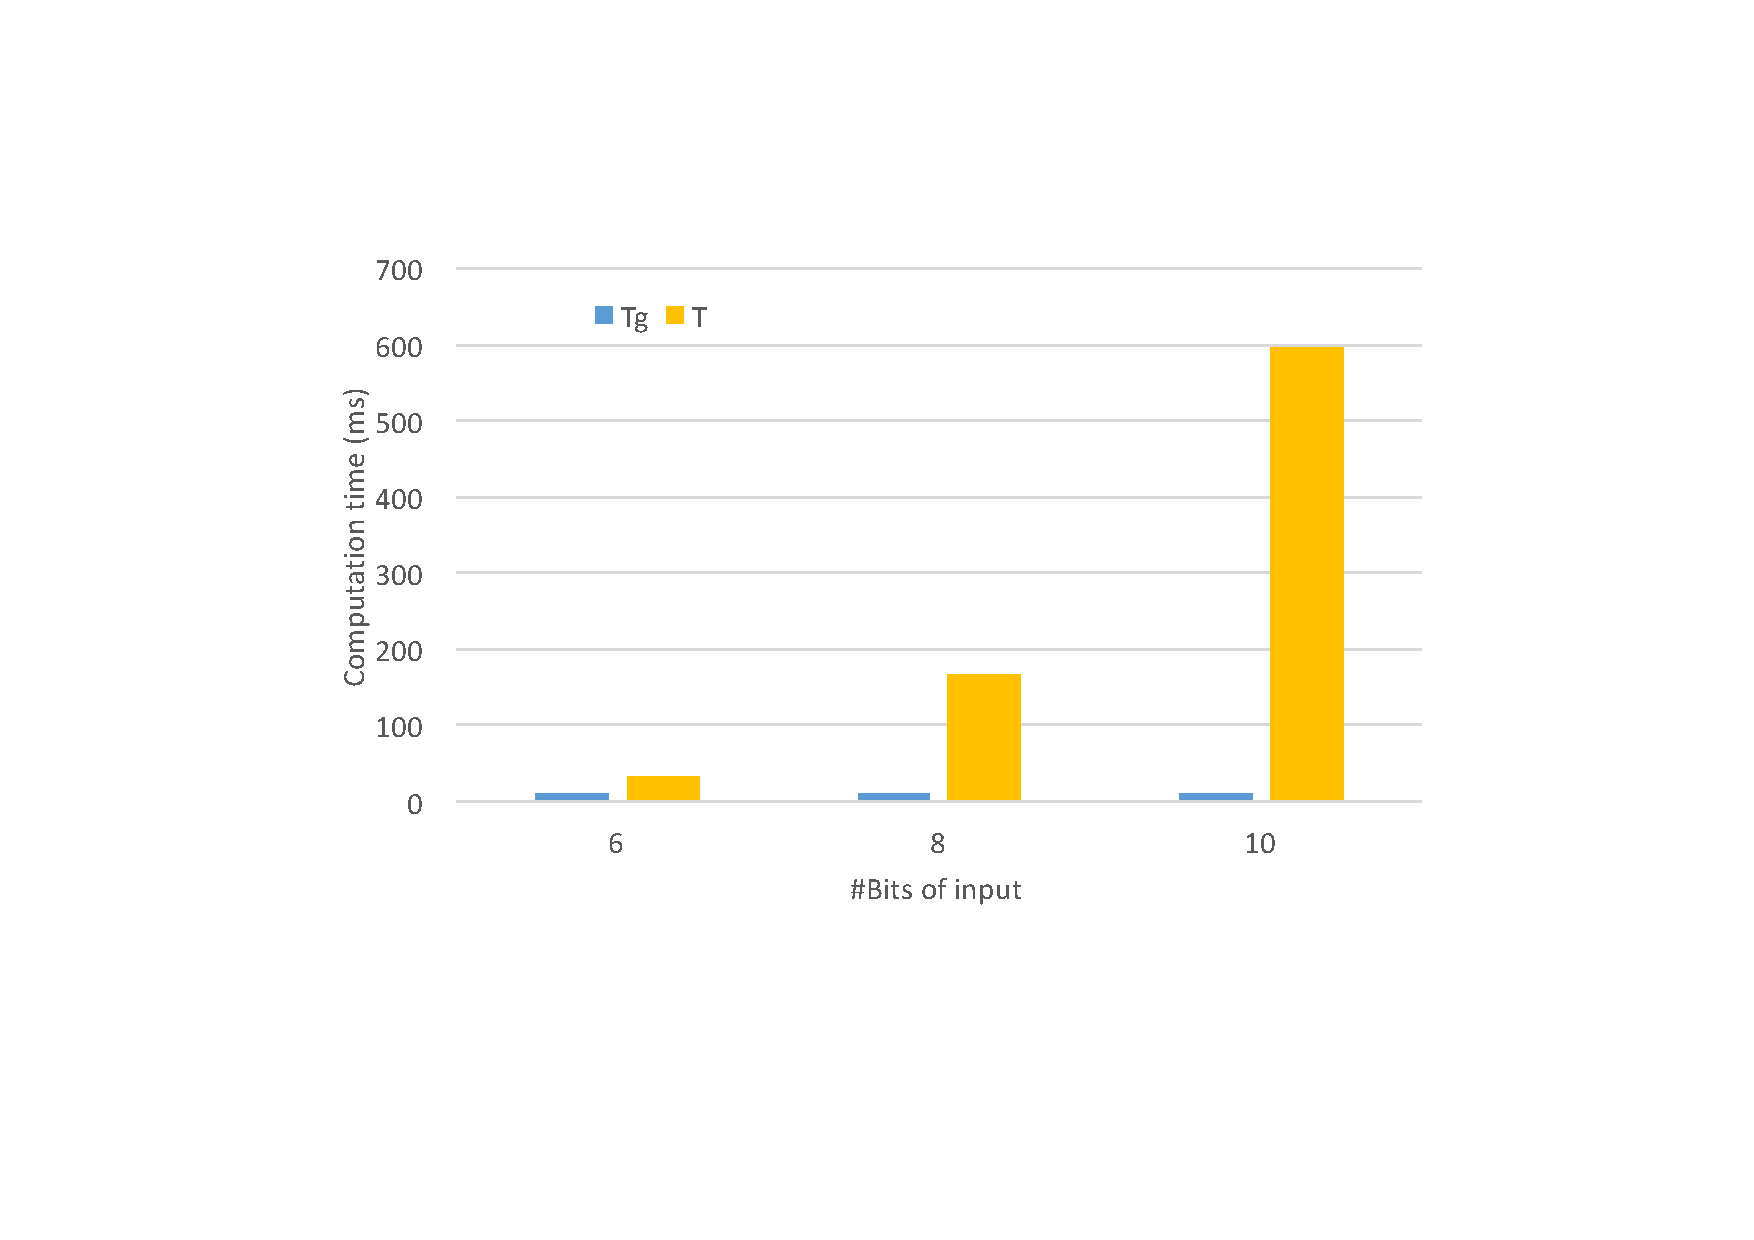
\includegraphics[scale = 0.5]{figures/figure-eval-t1.pdf}
%\vspace{-3mm}
%    \label{fig:e2-figure}
%    \centering
%    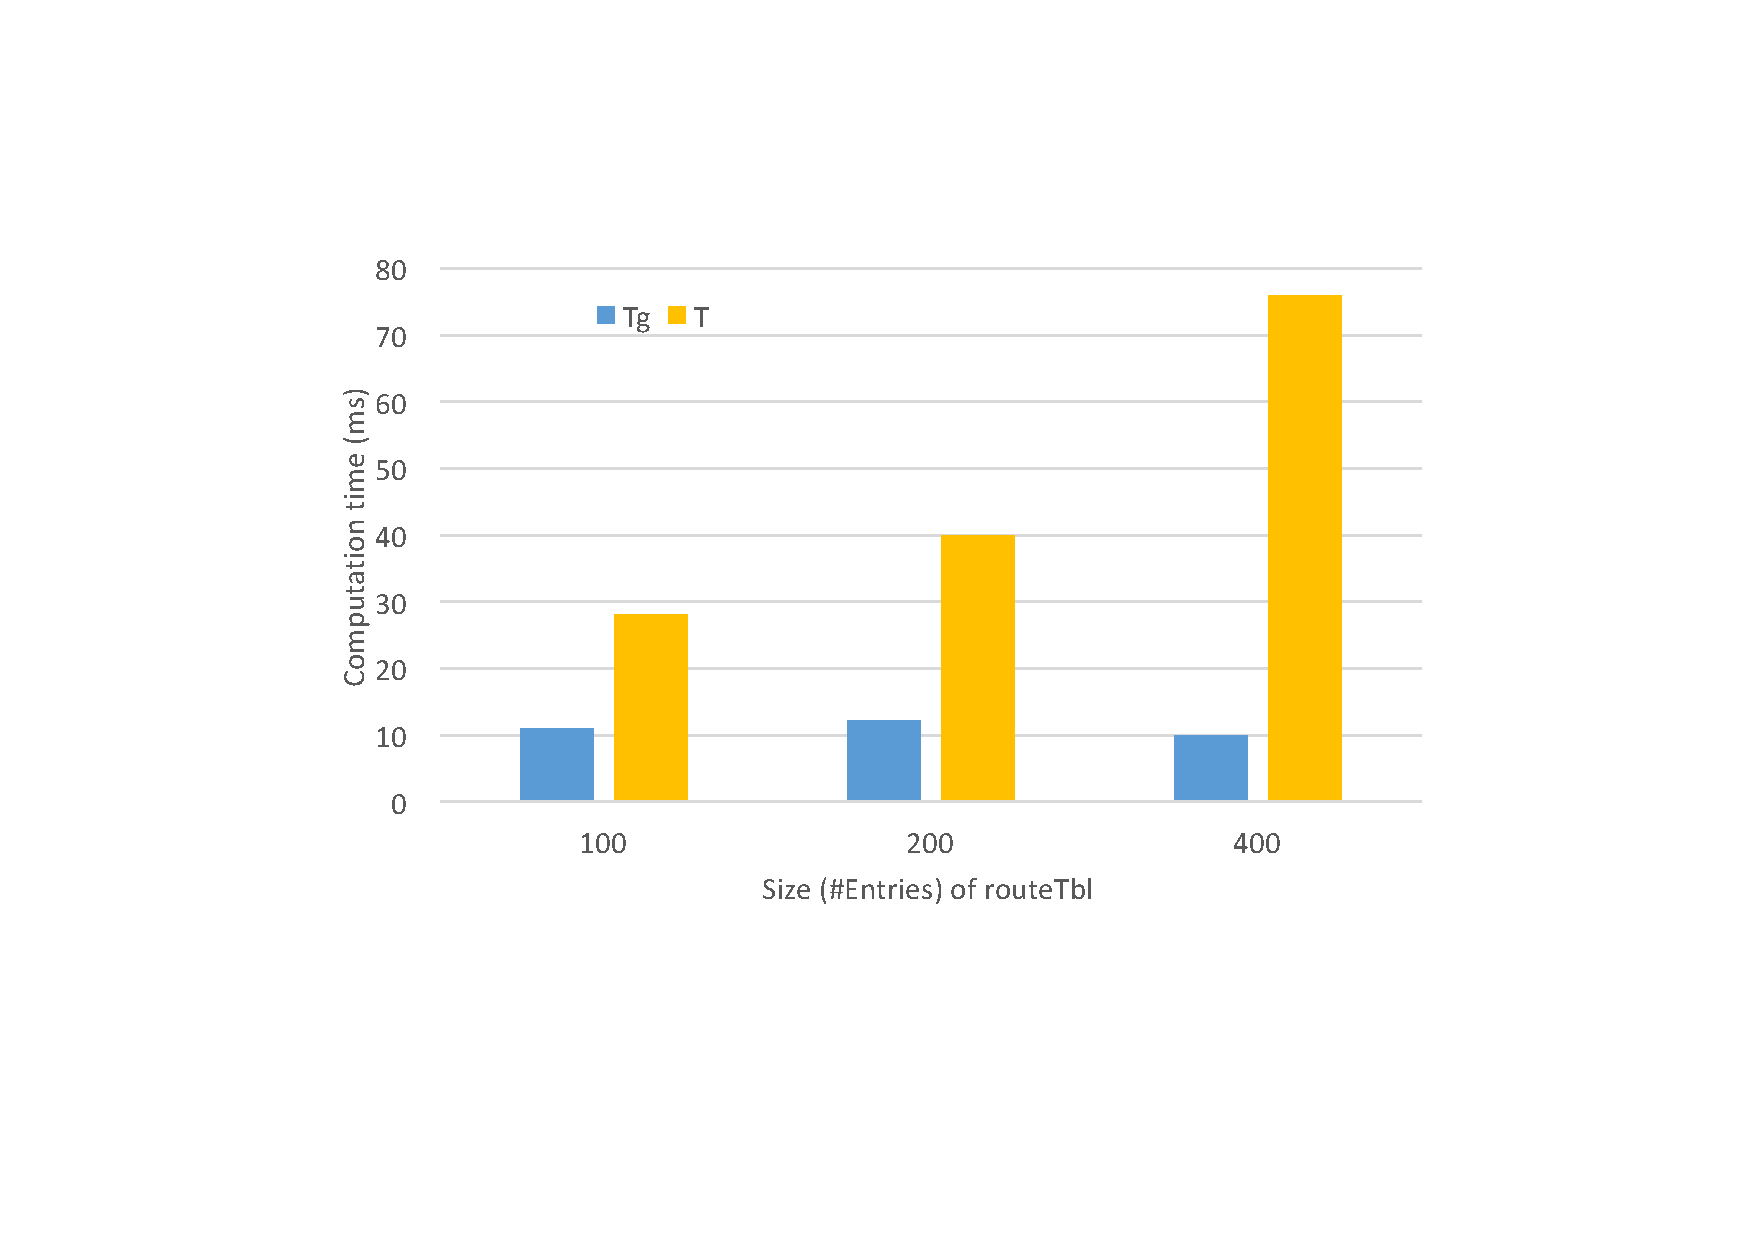
\includegraphics[scale = 0.5]{figures/figure-eval-t2.pdf}
%\vspace{-3mm}
%    \caption{Computation time required to generate $\tau(\texttt{simpleRoute})$ and $\tau_G(\texttt{simpleRoute})$ as input bit length varies.}
%    \label{fig:e2-figure}
%\end{figure}


\begin{figure}
  \centering
  \subfigure[Input size]{
    \label{fig:eval-ct:a} 
    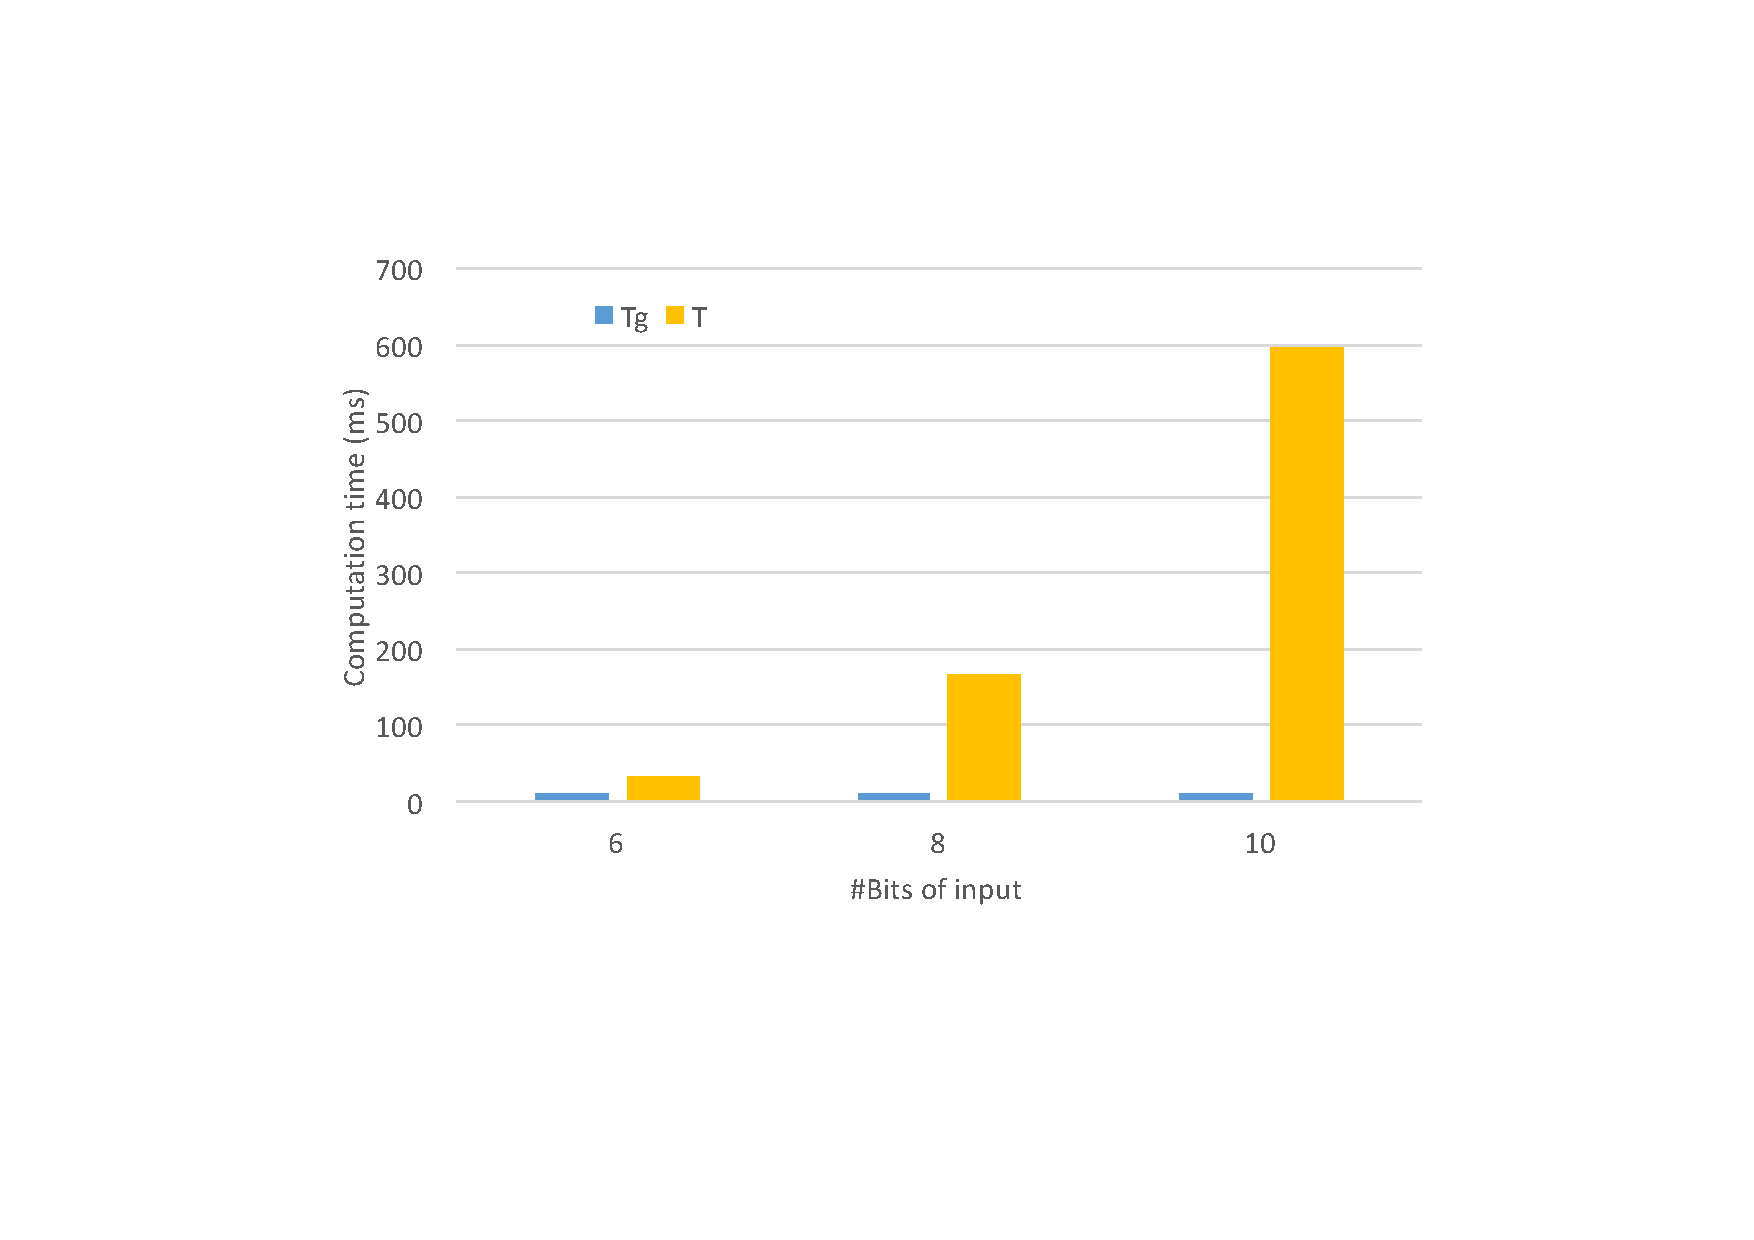
\includegraphics[width=0.4\textwidth]{figures/figure-eval-t1.pdf}}
  \hspace{1in}
  \subfigure[Table size]{
    \label{fig:eval-ct:b}
    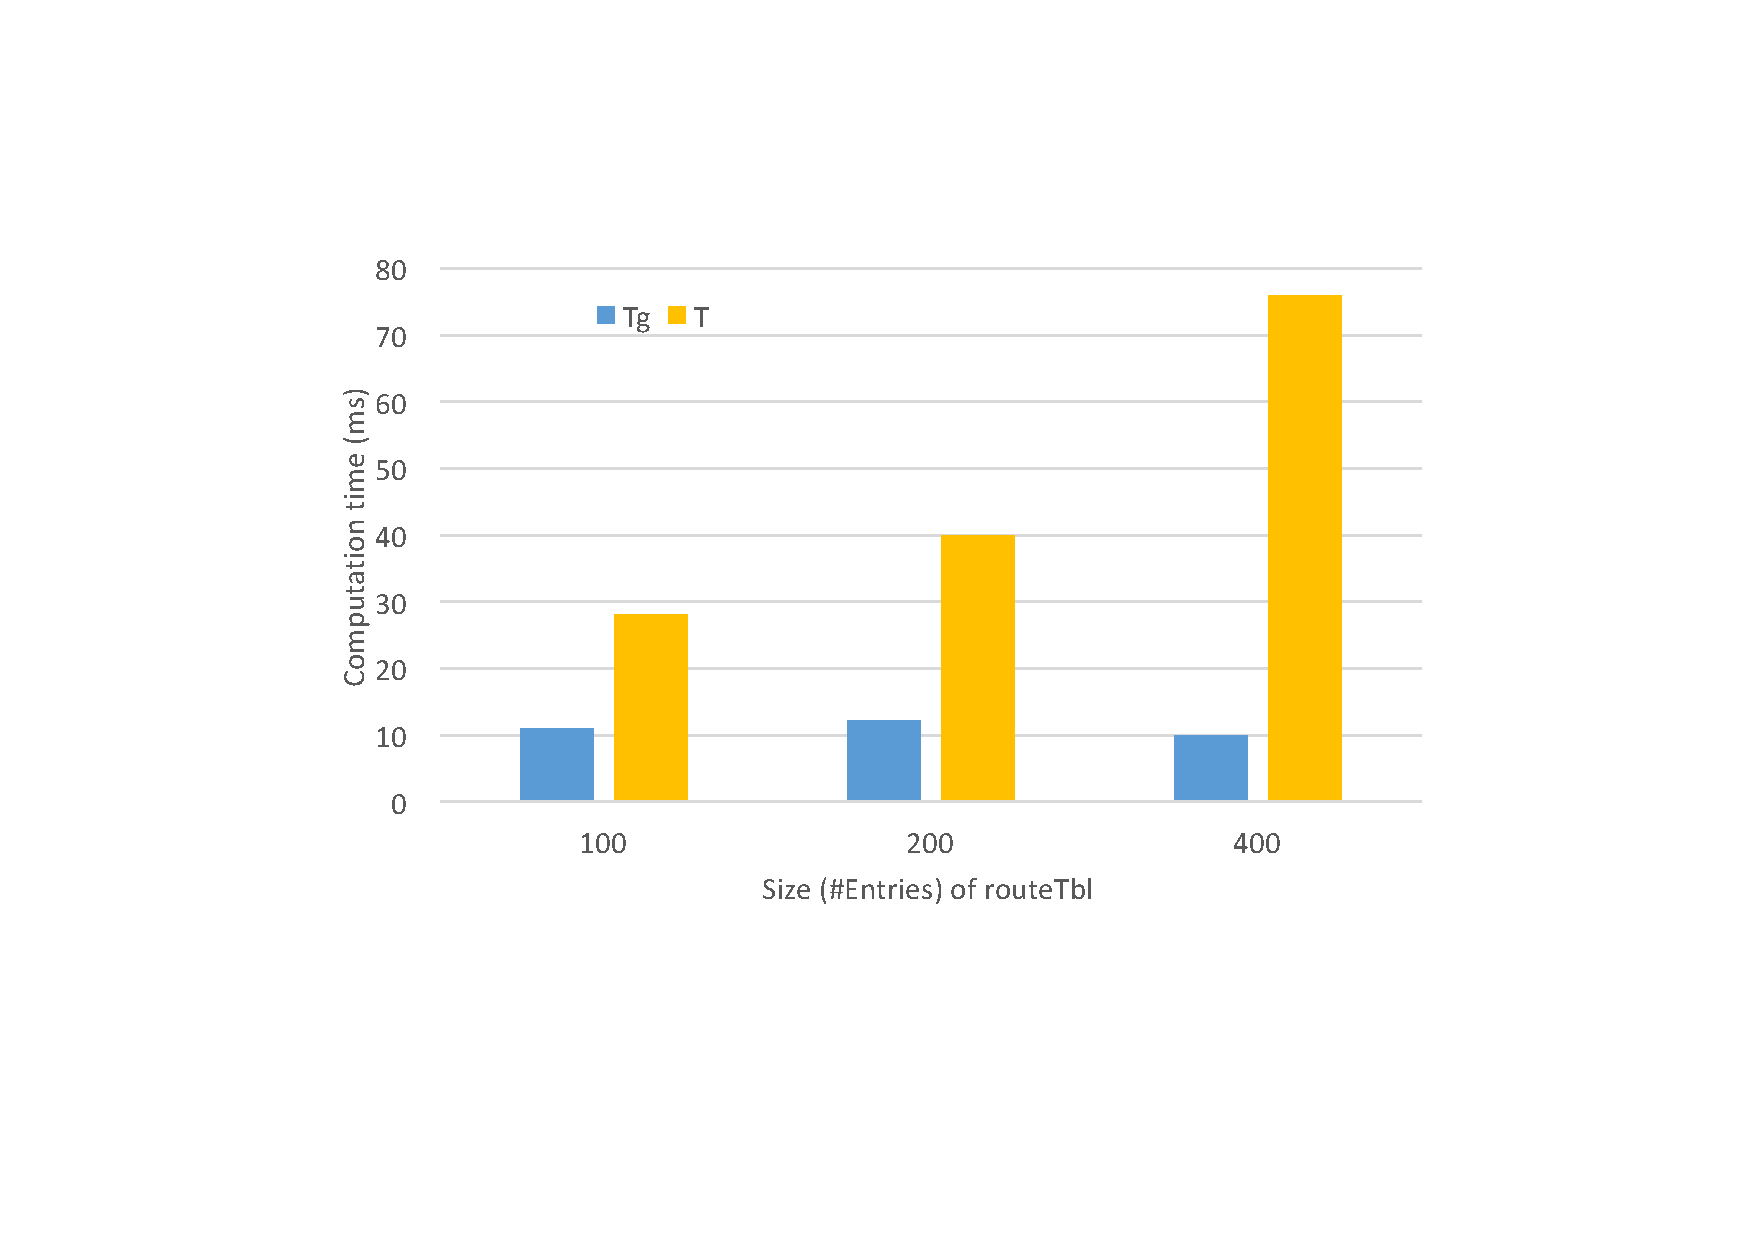
\includegraphics[width=0.4\textwidth]{figures/figure-eval-t2.pdf}}
  \caption{Computation time required to generate $\tau(\texttt{simpleRoute})$ and $\tau_G(\texttt{simpleRoute})$ as input bit length varies and the size of table varies.}
  \label{fig:eval-ct}
\end{figure}

\subsection{Characterization of a Pipeline}

%We now examine the memory utilization and computation time of pipeline characterization. We evaluate the following pipelines:

We now examine the characterization of a pipeline by evaluating the computation time and compactness of characterization functions of several pipelines. The compactness of a characterization function of a pipeline represents the output memory utilization of the characterization function compared with the size of all the possible $M$. We use the following pipelines in the evaluation:

\begin{enumerate}
  \item \textbf{The OF-DPA Abstract Switch 2.0:} The OpenFlow Data Plane Abstraction Abstract Switch 2.0 (OF-DPA) is an abstract switch model based on the Open Flow 1.3.4 protocol designed to allow the programming of Broadcom-based switches under the OpenFlow protocol. We examine two OF-DPA flow table configurations: bridging and routing (BR), and data center overlay tunnel (OT), which contain 7, and 3 tables in 5, 3 stages respectively.~\cite{OF-DPA}

  \item \textbf{PicOS:} PicOS is a network operating system for white box switches that provides OF programmability across HP, Edgecore and Pica switches. We examine two fixed pipelines offered by PicOS as table type patterns: PicOS's IP routing pipeline (IPR) and Policy routing pipeline (PR), which contain 4 and 5 tables in 4 and 5 stages respectively.~\cite{PicOS}
\end{enumerate}

\para{Results:} Table~\ref{tbl:table3} gives our characterization results for our evaluated pipelines. It shows the characterization results of several pipelines including four real pipeline structures and the example pipeline, \exampledp. We say a set of packet match fields $M$ is valid in a pipeline $p$ means the value of $\kappa_\rho(\rho)(M)$ can be computed by the first formula in the definition of $\kappa_\rho(\rho)(M)$. The results show that despite the theoretically large number of subsets of $\mathcal{M}$ across evaluated pipelines, memory utilization and computation time are small.

\begin{table}[t]
\centering
\scalebox{0.8}{
\begin{tabular}{ | l | l | l | l | l | }
    \hline
    Pipeline & \#Paths & Time (ms) & \#Valid $M$ & \#$M$ \\
    \hline
    \exampledp & 3 & 8 & 6 & 22 \\
    PicOS BR & 4 & 13 & 19 & $3*(2^{24})+2^7$ \\
    PicOS OT & 2 & 7 & 5 & $2^{24} + 16$ \\
    Broadcom IPR & 1 & 7 & 4 & $2^7$ \\
    Broadcom PR & 3 & 9 & 14 & $2*(2^{24})+2^7$ \\
    \hline
  \end{tabular}
  }
\vspace{2mm}
\caption{Characterization results of pipelines.}
\label{tbl:table3}
\end{table}

\subsection{Realization}

We now evaluate the percentage of successful realization of a function in a pipeline to see the factors of successful realization. We consider the example function \texttt{onPkt} with different content of tables. Specifically, for tables \texttt{condTbl} and \texttt{hostTbl}, we set the number of output values of tables ranging from 10 to 30 randomly, which means the domain size of \texttt{dstCond} and \texttt{dstSW} is from 10 to 30 (\ie, the average domain size is 20). For the pipeline side, we randomly decide the number of tables (from 2 to 4) of a pipeline and the length of bits of registers (from 4 to 10) for each table. Also, we set the match fields of the generated pipeline must contain the five match fields required by \texttt{onPkt} and each match field can only appear in one table. Then, we compute the successful realization percentage of \texttt{onPkt} and the generated pipeline by using the realization theorem.

\begin{figure}
  \centering
  \subfigure[\#Tables = 2]{
    \label{fig:eval-rp:a} %% label for first subfigure
    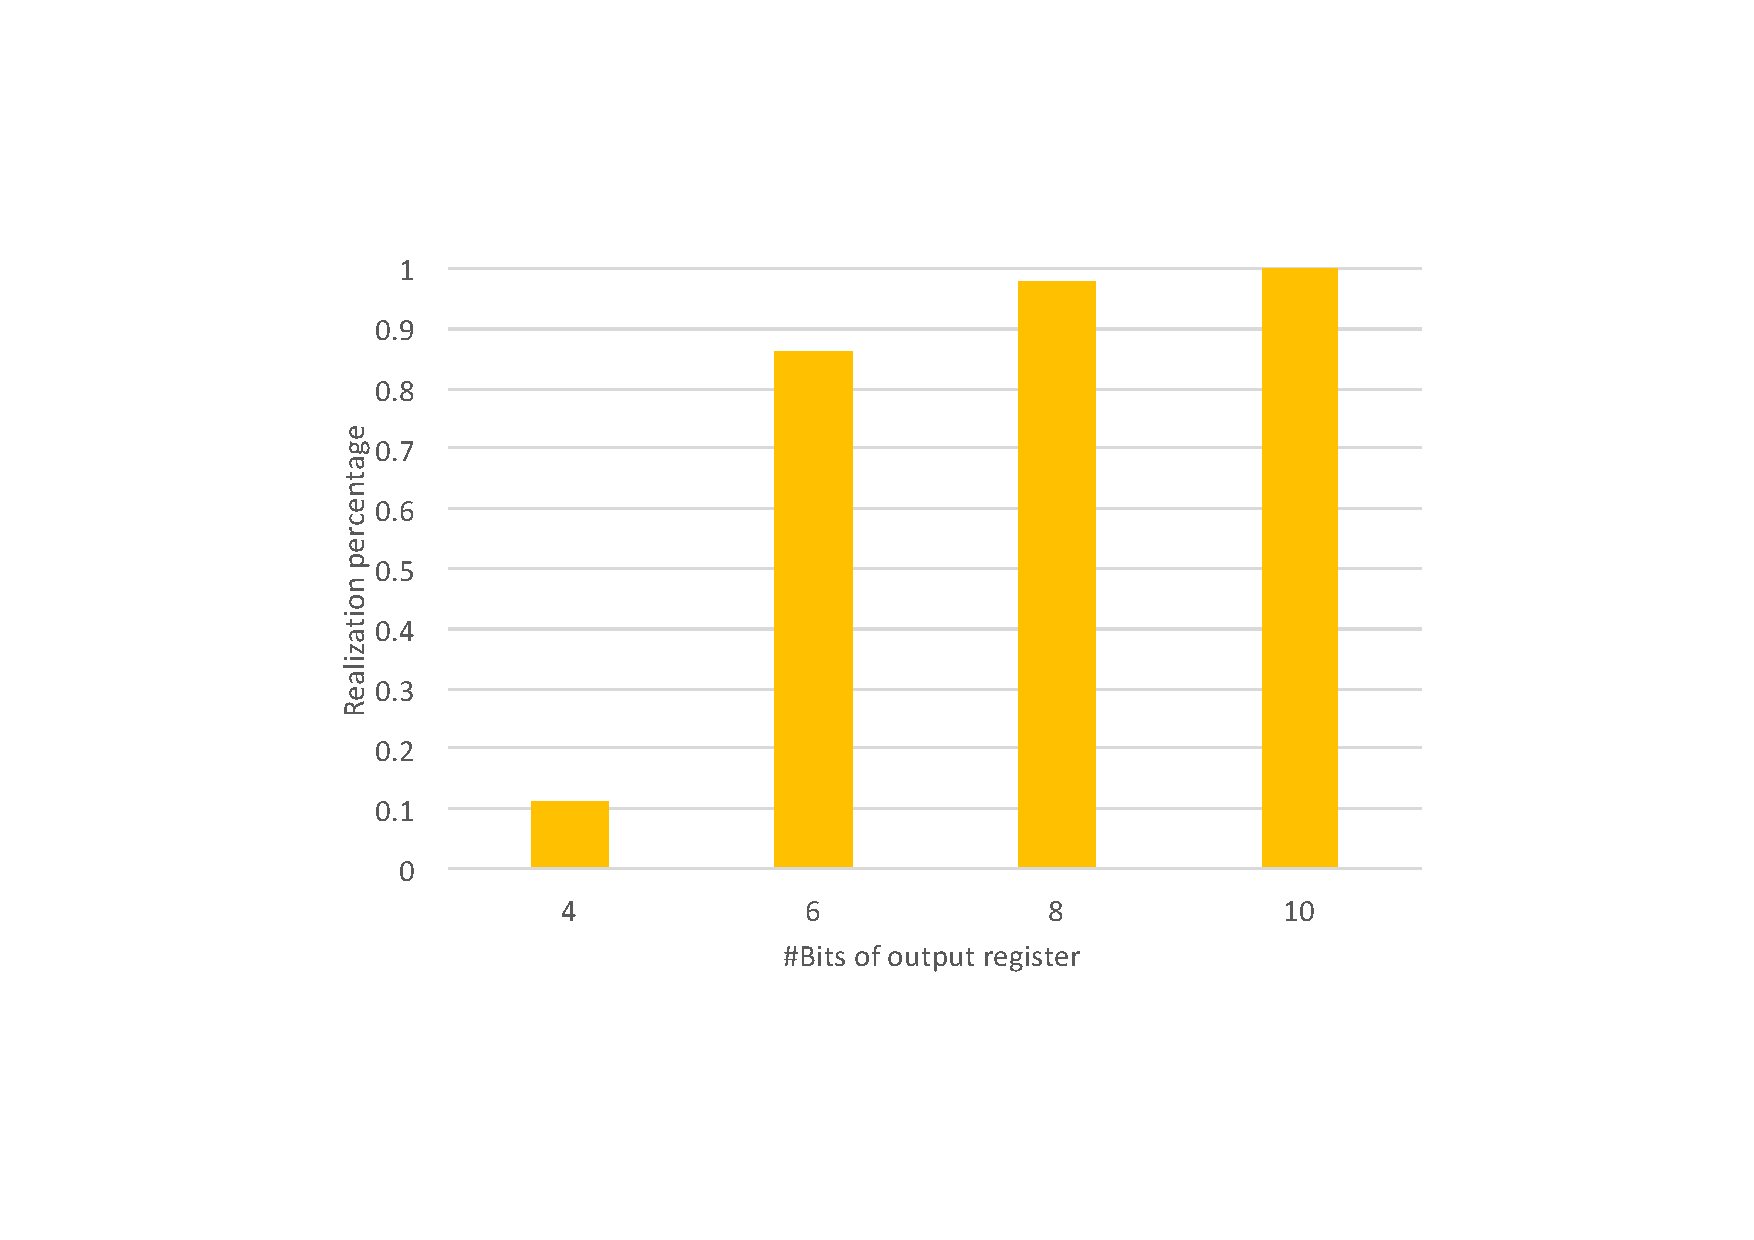
\includegraphics[width=0.4\textwidth]{figures/figure-eval-rp-2.pdf}}
  \hspace{1in}
  \subfigure[\#Tables = 3]{
    \label{fig:eval-rp:b} %% label for second subfigure
    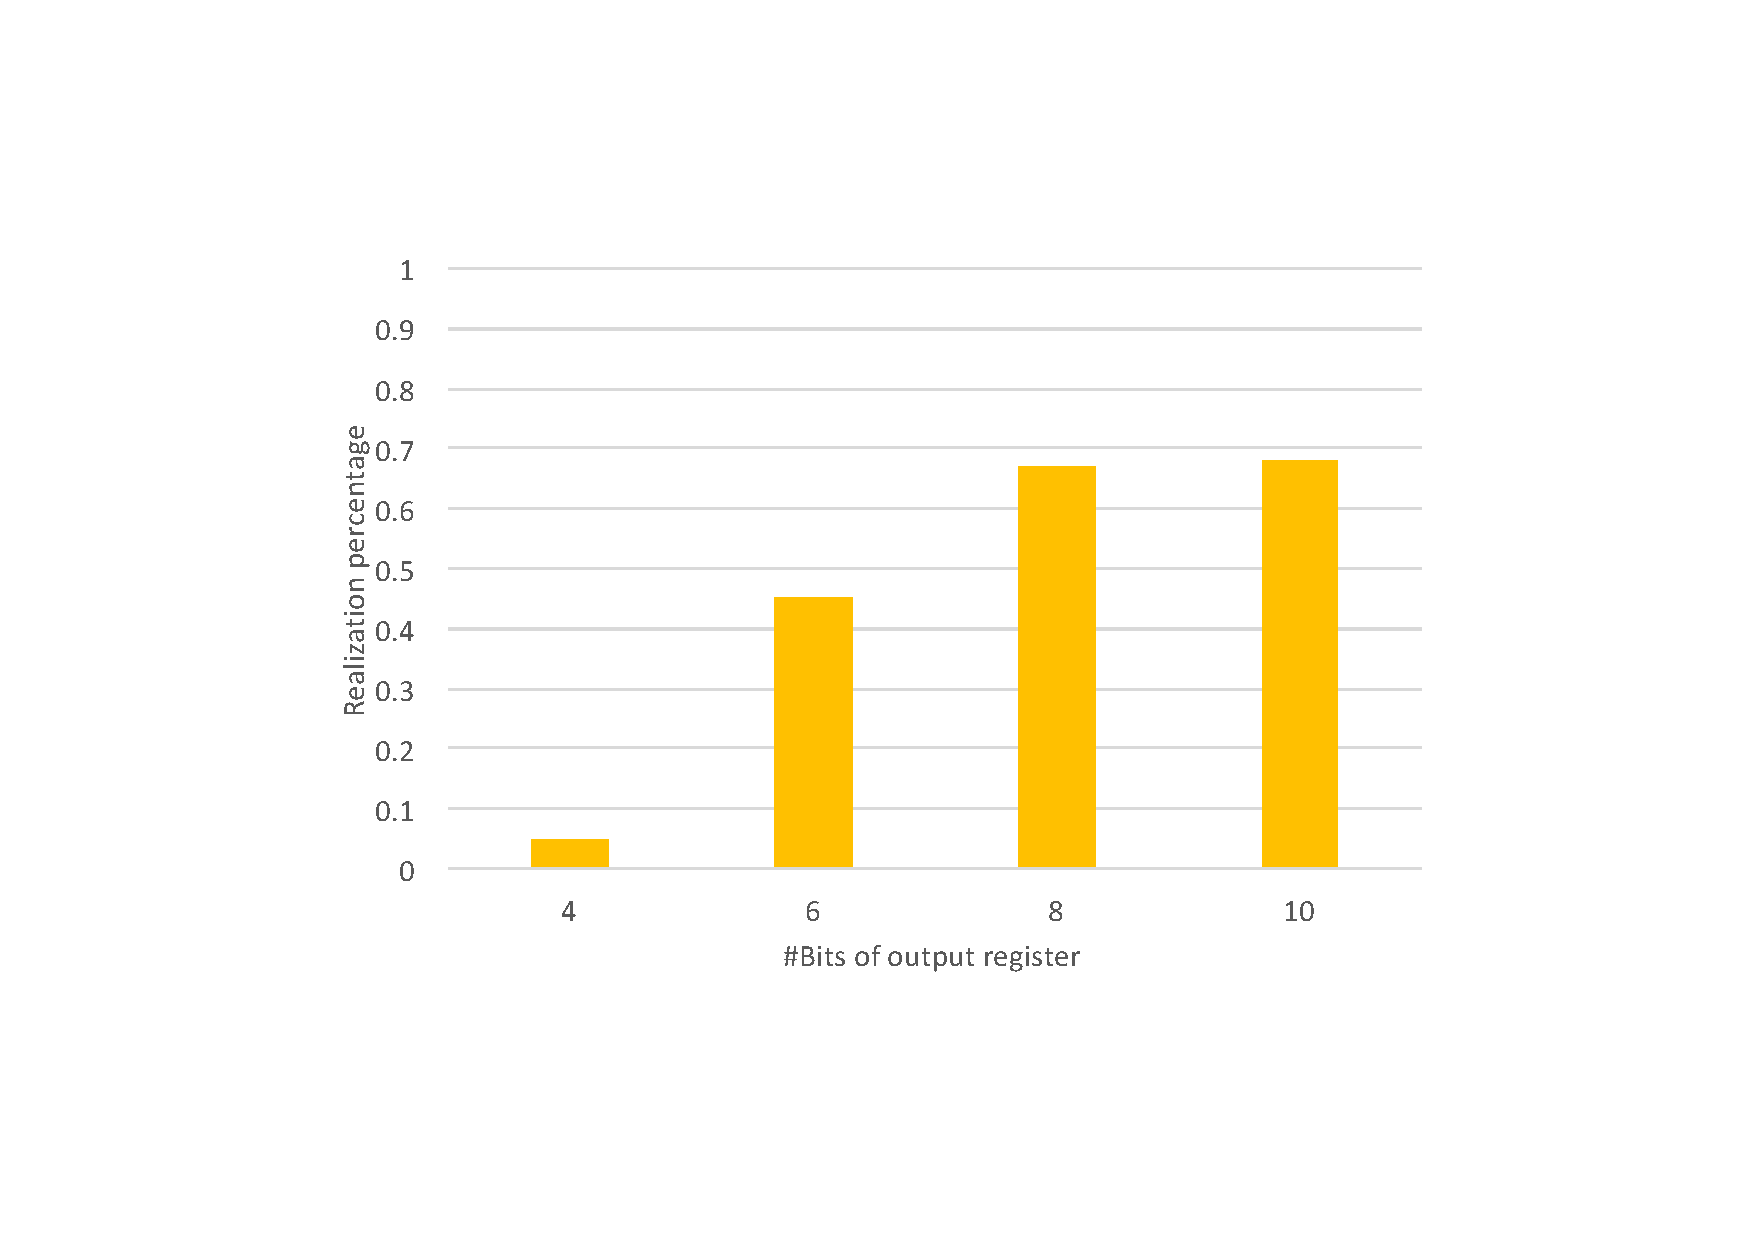
\includegraphics[width=0.4\textwidth]{figures/figure-eval-rp-3.pdf}}
  \subfigure[\#Tables = 4]{
    \label{fig:eval-rp:c} %% label for second subfigure
    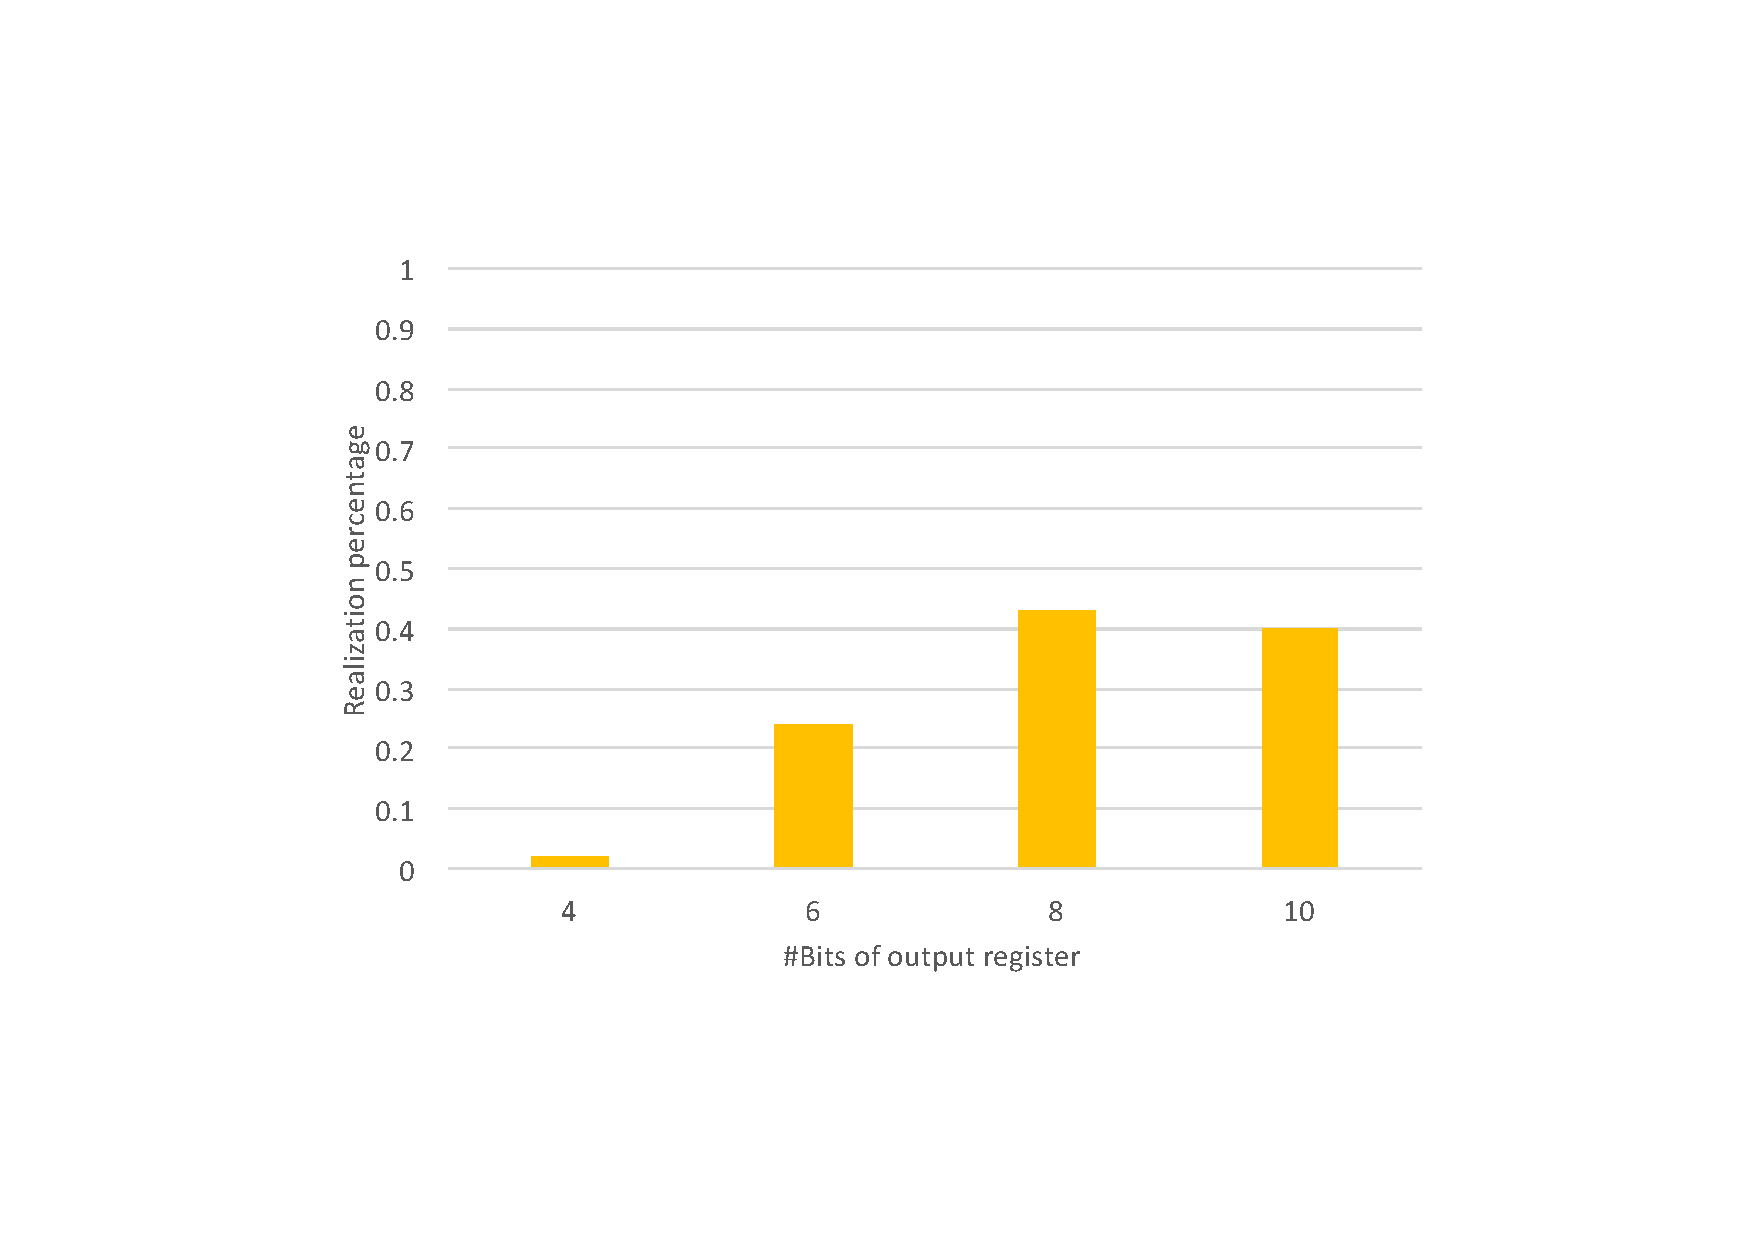
\includegraphics[width=0.4\textwidth]{figures/figure-eval-rp-4.pdf}}
  \caption{The percentage of realization for different number of tables and different length of registers.}
  \label{fig:eval-rp} %% label for entire figure
\end{figure}

\para{Results:} The result is shown in Fig.~\ref{fig:eval-rp}. Specifically, Fig.~\ref{fig:eval-rp:a} considers the pipeline with 2 tables; Fig.~\ref{fig:eval-rp:b} considers the pipeline with 3 tables; Fig.~\ref{fig:eval-rp:c} considers the pipeline with 4 tables. For each case, we compute the successful realization percentage with different length of bits of registers for each table. From the result of Fig.~\ref{fig:eval-rp:a}, we can find that a pipeline with more bits of registers can realize a function in a higher percentage. However, when the length is larger than a threshold, the successful realization percentage does not increase much. The threshold is determined by the size of domain of variables in the function. As shown in Fig.~\ref{fig:eval-rp:a}, the gap of successful realization percentage between 4 bits and 6 bits of length of registers (\ie, the available size of equivalent classes from 16 to 64) can be explained by the fact that the average domain size of variables (\ie, 20) is in the range between 16 and 64.

Furthermore, we can find the structure of pipelines also determines the realization percentage. A pipeline with 2 tables (\ie, there is no branch in the pipeline) has a relatively high successful realization percentage, while a pipeline with 3 or 4 tables which may contain branches has a low realization percentage as the structure of the pipeline is not well organized (\ie, the random mapping between matches fields and tables).

%The results show that despite the theoretically large number of subsets of $\mathcal{M}$ across evaluated pipelines, memory utilization and computation time are small. It shows the characterization results of several pipelines including four real pipeline structures and the example pipeline, \exampledp. We say a set of packet match fields $M$ is valid in a pipeline $p$ means the value of $\kappa_\rho(\rho)(M)$ can be computed by the first formula in the definition of $\kappa_\rho(\rho)(M)$.  The result shows that though there are many combinations of $M$ for the output of characterization of a pipeline, the real memory utilization should be small. Also, it shows the computation of pipeline characterization is very fast.

%
%The goal of our evaluation is to demonstrate that the pipeline capacity theorem allows us to determine whether a generic program can be compiled to a fixed pipeline in a memory and time efficient manner for state-of-the-art programs and hardware. We then discuss a range of usage scenarios that our theorem enables. %All experiments are conducted on a processor Intel Core i5 running at 1.6 GHz, with 4 GB RAM and running OS X system. 
%
%\subsection{Setup, Pipelines and Programs}
%All experiments are conducted on a single processor 10-core (20-virtual thread) Intel(R) Xeon(R) CPU E5-2650 v3 machine running at 2.3 GHz, with 64GB RAM and running 64 bit Fedora Linux 24.
%
%
%\para{Pipelines:} We use the following pipelines in our experiments.
%
%\begin{enumerate}
%  \item \textbf{The OF-DPA Abstract Switch 2.0:} The OpenFlow Data Plane Abstraction Abstract Switch 2.0 (OF-DPA) is an abstract switch model based on the Open Flow 1.3.4 protocol designed to allow the programming of Broadcom-based switches under the OpenFlow protocol. We examine 3 OF-DPA flow table configurations: bridging and routing, data center overlay tunnel, and VPWS, which contain 17, 9, and 15 tables in 8, 5, and 12 stages respectively.~\cite{OF-DPA}
%
%  \item \textbf{PicOS:} PicOS is a network operating system for white box switches that provides OF programmability across HP, Edgecore and Pica switches. We examine two fixed pipelines offered by PicOS as table type patterns: PicOS's IP routing pipeline and Policy routing pipeline, which contain 7 and 8 tables in 5 and 6 stages respectively.~\cite{PicOS}
%\end{enumerate}
%
%\para{Programs:} Further, we test the following programs in our experiments:
%
%\begin{enumerate}
%\item\textbf{Program 1:}
%\end{enumerate}
%
%\subsection{Capacity vector calculation}
%
%\subsection{Transmission vector calculation}
%
%\subsection{Capacity transmission vector comparison}